\documentclass[a4paper,12pt]{article}
\usepackage{listings}
\usepackage{graphicx}
\usepackage{subcaption}
\usepackage{minted}
\title{Solar room heating automation}
\begin{document}
\maketitle
\begin{abstract}
    A project to find a cheap and simple way to heat houses.
\end{abstract}
\tableofcontents
\section{Introduction}

In Britain, many people face the issue of freezing due to the inability to heat. 
Indoor heating is a massive energy consumer in the UK, responsible for about 20\% of greenhouse gas emissions\cite{url:energyUse}. 
This not only contributes to climate change but also leads to unsustainable expenses for households who need to heat during winter.

The aim of this project is to develop a device that permits people to make more use of solar energy to heat their rooms, 
while still keeping the cost of hardware and installing the system low. 

The potential of using solar energy is significant, about $1.3 KW/m^2$ \cite{url:solarConstant}. 
Even if the majority of the energy is lost to its surroundings and only $500 W/m^2$ are captured, 
this may save up to $5 Kwh$, or the equivalent of 1 Kg of firewood for each $m^2$ of a south-facing window. 

\subsection{Photovoltaics for room heating}

An obvious choice to start with would be photovoltaic panels, using the generated electricity to heat the water used in the heaters, 
but a cursory market study of available components indicates that an adequately sized photovoltaic system (roughly 2kW of power) 
would cost roughly £4000\cite{url:solarEnergyStore}, well above the budget of typical persons in need of additional heating  
and with an unclear amortisation schedule. 
Therefore, we rule out using photovoltaics for electric heating.

\subsection{Air collectors for room heating}

Another method that was considered was using Air collectors for room heating, which work by using solar energy to heat the air, which is then circulated into a room. 
They are simple and robust as well as providing fresh air to the room, ensuring the house does not grow moist when the owner is away for longer periods. 
However, they are very expensive at roughly £2200 for 2kW heating output\cite{url:solarVenti}. Also, they are difficult to install and often only ideal for a permanent home, 
so those renting a house - generally those who require it the most - would be unable to make use of it.

\subsection{Window insulation}

A very cost effective way of keeping the temperature up in a room is to open curtains when the sun is heating the space through the window, 
and then close the curtains when the temperature starts to fall again in the evening. 
The issue with this is that many people are away at work during the optimal time for closing the curtains.

For this reason, we decided that the most prudent course of action for this project is to design a system that automatically closes the curtains at the optimal time, 
letting the sun in only while it still effectively heats. 

In addition, this system is very simple and cheap, which would allow those who need this extra insulation to afford it.

The system we designed closes the curtains when the sun goes away or the temperature in the room starts to drop, so as to keep the solar heat inside 
and reduce heating costs.

It has a detector that can sense very bright light (i.e., the sun), a sensor to measure the temperature accurately and an actuator to 
release a curtain closing mechanism, which is triggered when the sun has vanished for a certain time or becomes too weak to effectivly heat the room.
 The system does not respond immediately, so that wrong measurements or reappearance of the sun do not result in reduced energy harvesting.


For cost reasons, the system does not support opening curtains automatically, as originally considered. Instead, the user needs to reset these manually.
Closing works by releasing a weight with a servo arm. The potential energy of the weight moves the curtain via simple pulleys.

Subsequent to closing action, the locking mechanism moves back into the original position for convenience in resetting the weight and curtain 
to harvest solar energy.

\section{Project Plan}

\subsection{Overview}

This paragraph outlines steps in implementing the project described in the previous section.

Table \ref{tab:projtimeline} lists the various steps required in this project and their deadlines, along with the dates for other competitions this project was submitted in.

\begin{table}[h!]
    \caption{Project timeline}
    \begin{tabular}{l | r}
        Work package & Due date \\
        \hline
        Formulate problem &  8 January 2025 \\
        Research suitable sensors & 13 January 2025 \\
        Log data provided by sensors & 20 February 2025 \\
        Plot data & 22 March 2025 \\
        Develop algorithm for curtain closing time & 23 March 2025 \\
        Build hardware & 23 March 2025 \\
        Create video presentation & 24 March 2025 \\
        Submit to Raspberry Pi competion to get feedback & 24 March 2025 \\
        Write project report, submit to CREST &  31 June 2025\\
    \end{tabular}
    \label{tab:projtimeline}
\end{table}

\subsection{Curtain Closing mechanism}

\begin{figure}
    \centering
    \begin{subfigure}{0.3\textwidth}
        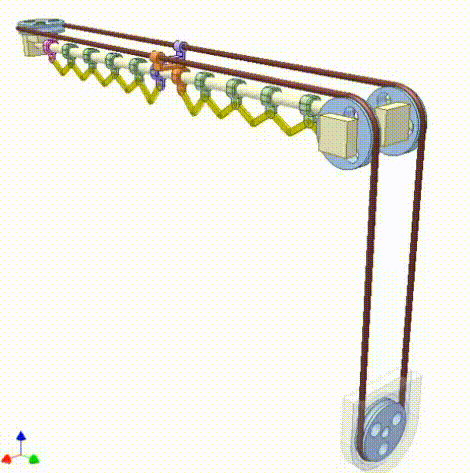
\includegraphics[width=\textwidth]{figures/initialCurtainMechanism1.png}
        \caption{Closed}
    \end{subfigure}
    \hfill
    \begin{subfigure}{0.3\textwidth}
        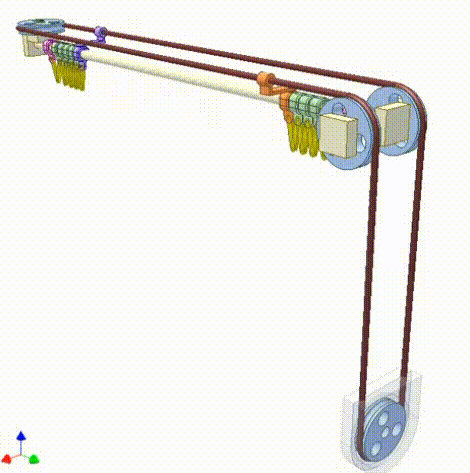
\includegraphics[width=\textwidth]{figures/initialCurtainMechanism2.png}
        \caption{Open}
    \end{subfigure}
    \hfill
    \begin{subfigure}{0.3\textwidth}
        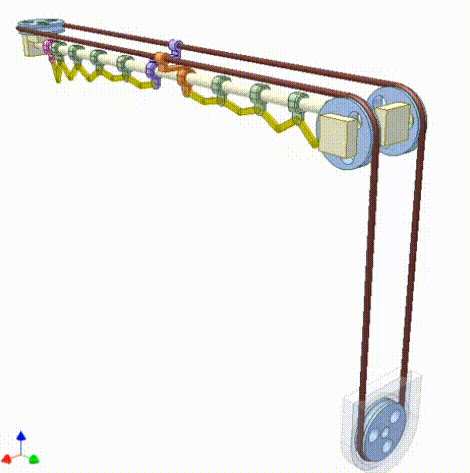
\includegraphics[width=\textwidth]{figures/initialCurtainMechanism3.png}
        \caption{Closed again}
    \end{subfigure}
    \caption{Mechanism for opening and closing curtains, requiring several pulleys, connectors and a stepper motor \cite{url:initialCurtainMechanism}. 
    DC motor attached to a pulley spins when activated, moving the curtains attached to the pulley system.}
    \label{fig:initialCurtainMechanism}
\end{figure}

\begin{figure*}
    \centering
    \begin{subfigure}[][][]{0.5\textwidth}
        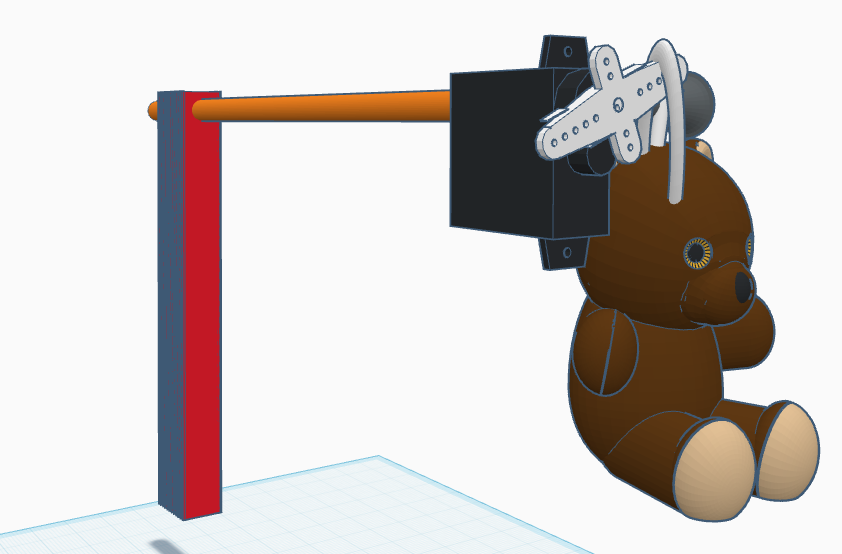
\includegraphics[width=\linewidth]{figures/curtainModelOpenFront.png}
        \caption{Open}
    %\end{subfigure}
    %\hfill
    %\begin{subfigure}[][][]{0.5\textwidth}
        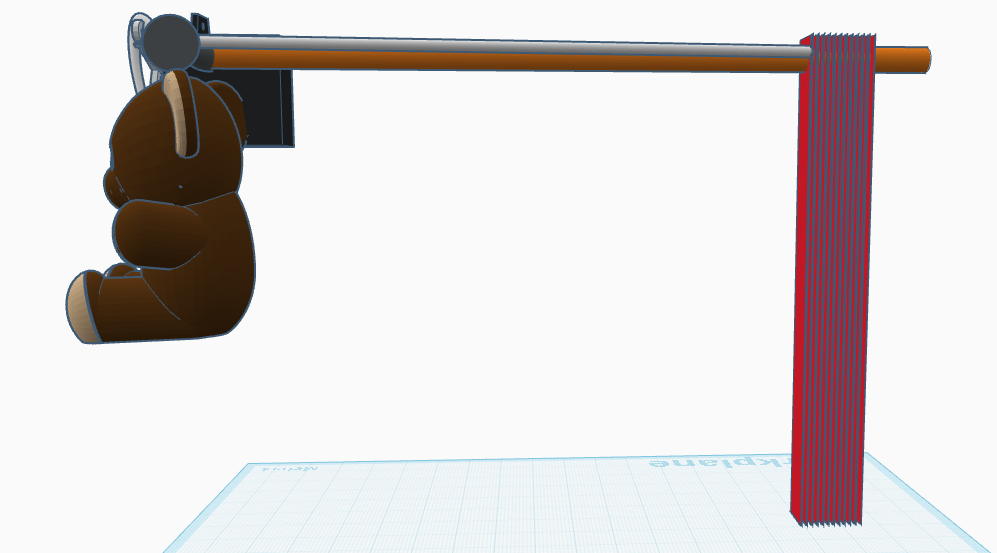
\includegraphics[width=\linewidth]{figures/curtainModelOpenSide.png}
        \caption{Open}
    %\end{subfigure}
    %\hfill
    %\begin{subfigure}[][][]{0.5\textwidth}
        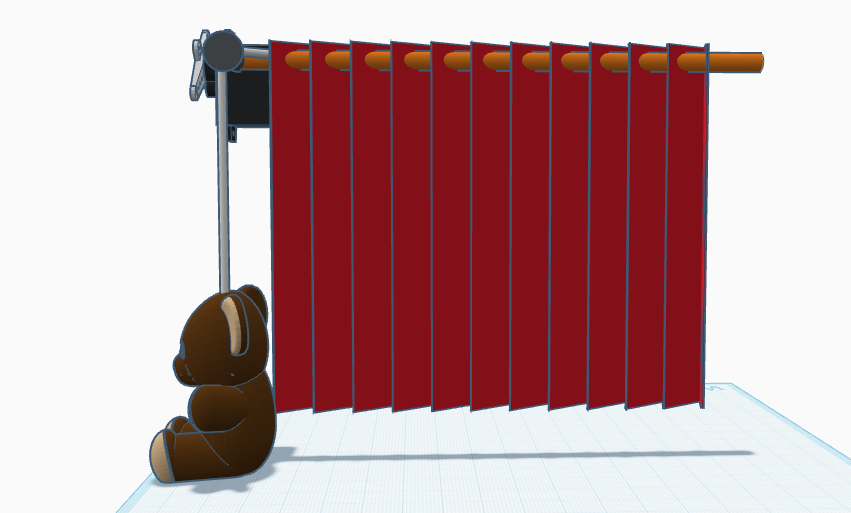
\includegraphics[width=\linewidth]{figures/curtainModelClosedSide.png}
        \caption{Closed}
    \end{subfigure}
    \begin{subfigure}[][][b]{0.4\textwidth}
        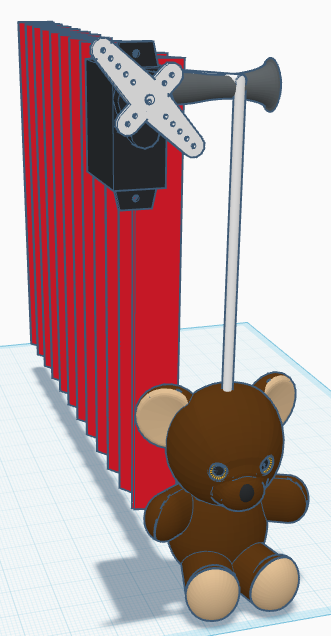
\includegraphics[width=\linewidth]{figures/curtainModelClosedFront.png}
        \caption{Closed}
    \end{subfigure}
 
    \caption{Curtain system: Open and closed state.}
    \label{fig:CurtainMechanismOpen}
\end{figure*}

One of the main challenges we faced was to design a mechanism that could close the curtains in a cheap and reliable way. 
An example of such a rather complex and costly system is shown in Figure \ref{fig:initialCurtainMechanism}.
We designed a similar system on a large curtain.

While seemingly simple at the start, the design quickly became less than ideal, as it would require additional sensors to signal the motor to stop, 
and the resistance between the curtain and the railing was so great that the pulley connected to the motor could not overcame it. Both of these problems were solvable, 
but the cost would be increased significantly, and so we designed a new system:

A weight would be connected to the curtain, to be released by a servo. The weight would fall and provide the energy to close the curtain. 
The user has to reset the curtain when the sun is about to heat the room again in the next morning. Although this system is only able to close curtains, 
it provides the cheap and simple option we needed, so we settled onto this version.

To reduce friction, we used fishing wire and a pulley. This allowed us to to roll the wire around the pulley several times, ensuring that it would not slip off. 
Our newtonmetre recorded that we needed roughly 0.4 N, the equivalent of an average size teddy bear. It worked perfectly first time, but for the pulley to hold, 
we required super glue as hot glue wasn't strong enough. Afterwards, the servo was attatched under it, to be connected to a loop at the bottom.


\subsection{Sensor selection criteria}

In order for the system to accurately judge the optimal time to close the curtain, external sensors would be required.
Selection criteria for sensors include:
\begin{itemize}
    \item Cost
    \item Robustness
    \item Measurement accuracy
    \item Simple to integrate
    \item Availability
\end{itemize}

The data it requires would be the amount of energy going into the room and the energy going out. Thus, our options were:

\begin{itemize}
    \item A temperature sensor - measure the temperature to determine when the temperature drops and ensure the Photoresistor does not act when the sun goes behind a cloud.
    \item A UV detector - measure the strength of the suns rays.
    \item A Photoresistor (A light sensor) - measure how bright it is, if the sun has gone down and to get a quicker reaction than the temperature sensor.
    \item A Photo Diode (A faster-responding light sensor) - as the Photoresistor.
\end{itemize}

\begin{table}[h!]
    \caption{Sensor trade study. 5 = perfect, o = terrible}
    \begin{tabular}{l | l | l | l | l | l}
        Sensor & Price & Availability & Accuracy & Simplicity & Total\\
        \hline
        Photo Resistor & 4 & 3 & 4 & 2 & 13 \\
        Temperature Sensor & 4 & 4 & 4 & 5 & 17 \\
        Photo Diode & 1 & 4 & 5 & 3 & 13 \\
        UV detector & 1 & 3 & 2 & 1 & 7 \\

    \end{tabular}
    \label{tab:sensor}

\end{table}

As seen in the trade study in Table \ref{tab:sensor}, the Temperature sensor, the Photo Diode and the Photo Resistor scored the highest points. 
While the Photo Diode would be very accurate, it is unneccessarily expensive when a Photoresistor would do just fine. 
A UV sensor has a high price and needs to be placed outside to work effectively, which would make the process of installing it too complicated. 
Therefore, we chose a Temperature Sensor and a Photoresistor as the sensors for the curtain system.

\subsection{Equipment}                                                                                                                                                                                                                                                                                                                                                                                                                                                                                                                                                              

Table \ref{tab:equipment} lists the parts that were required while building this project.

\begin{table}[h!]
    \caption{Equipment}
    \begin{tabular}{l | l | l}
        Parts & Price & Source \\
        \hline
        LDR Photo Resistor & £ 3.99 & Bought by Mr. Chikunga \\
        DS18B20 Temperature Sensor & £ 3.95 & Bought by Mr. Chikunga \\
        Servo Motor & £ 3.99 & Scavenged from a robot \\
        Arduino Nano & £ 4.99 & Scavenged \\
        Micro SD Card & £ 7.99 & Bought on Amazon \\
        Salvaged Parts & £ 1 & - \\
        Model Stand & 18.99 & Bought on Amazon \\
        Model Curtain & 10.19 & Bought on Amazon \\
        Total & £ 55.09 & - \\
    \end{tabular}
    \label{tab:equipment}
\end{table}

\section{Project Execution}

\subsection{Hardware Assembly}

\begin{figure}[h!]
    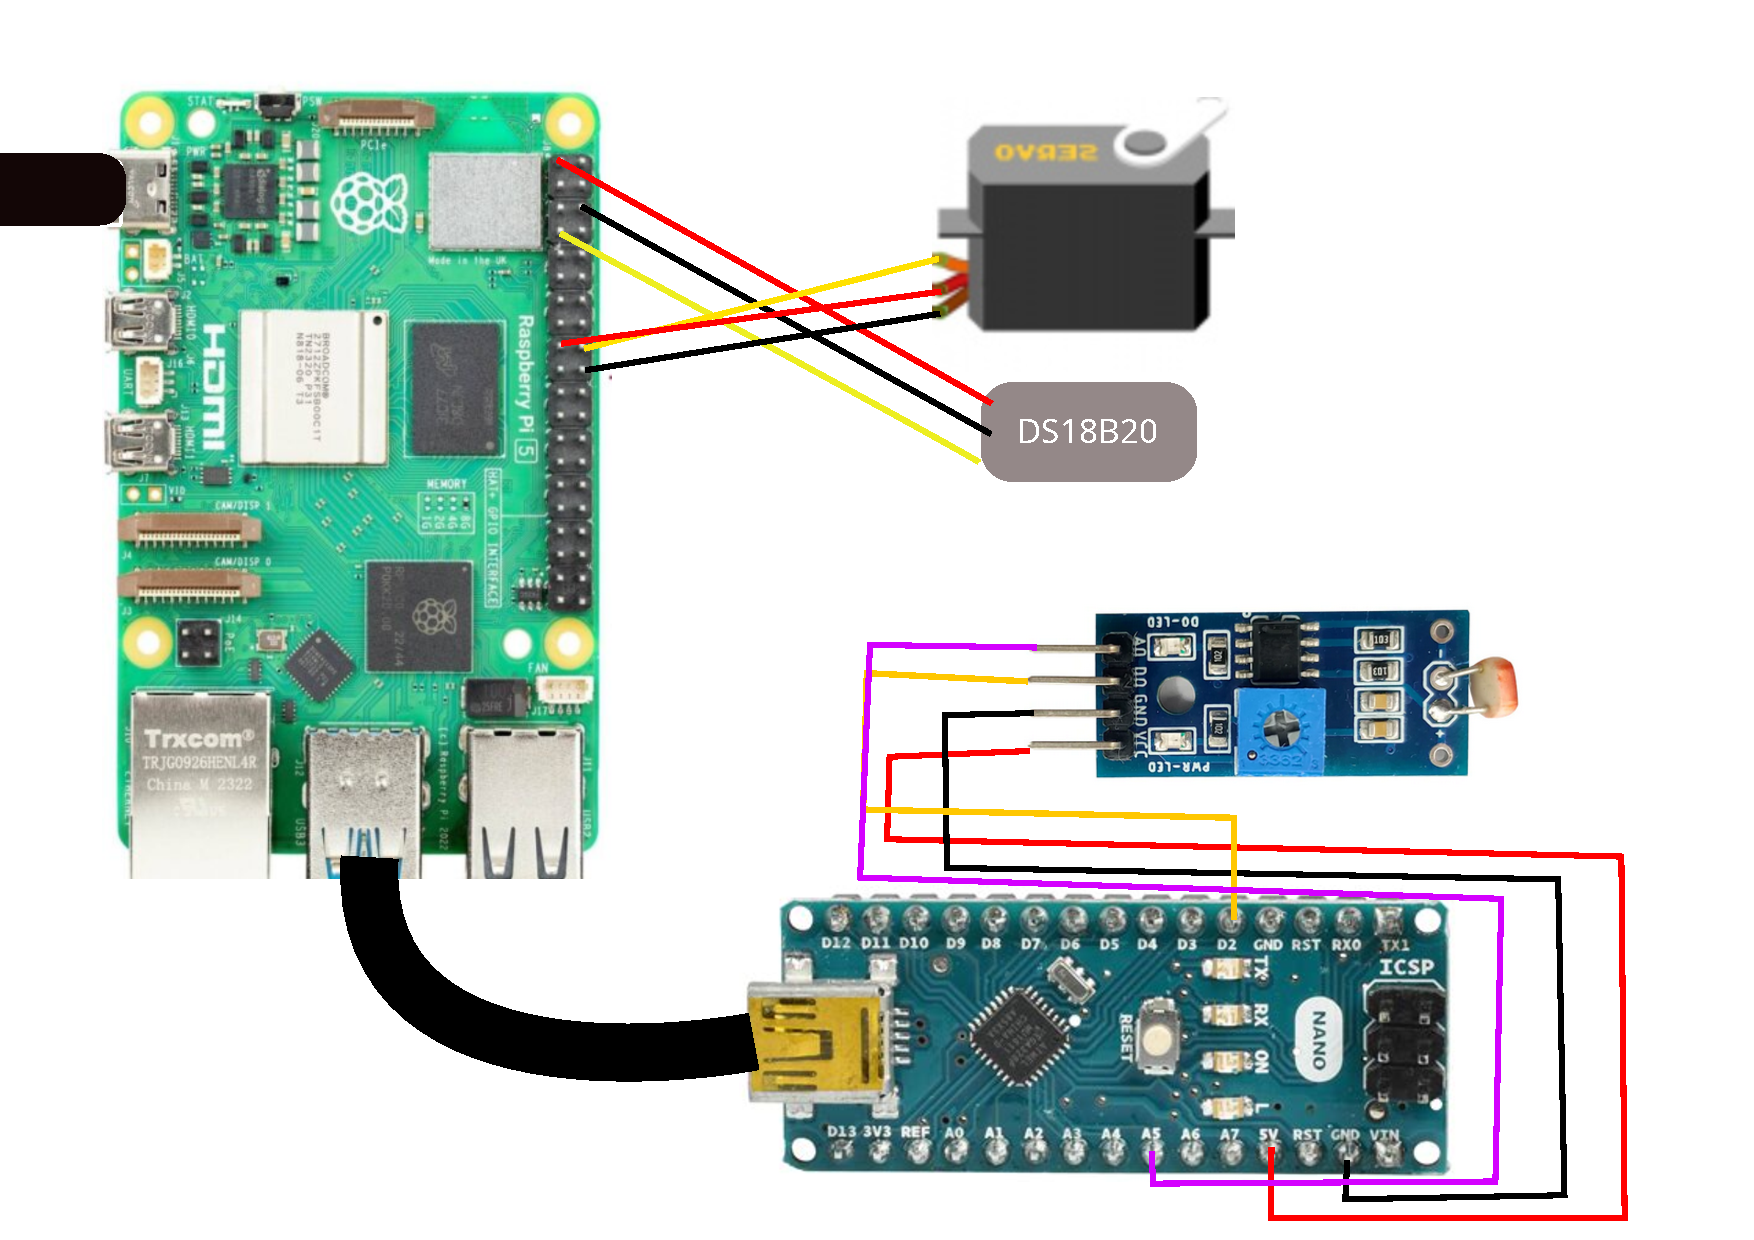
\includegraphics[width=\linewidth]{./figures/curtainCircuit.pdf}
    \caption{Electronics components of curtain closer. The Raspberry Pi computer directly controls the servo and reads from the digital temperature
    sensor DS18B20, while the photoresistor board for light level measurements needs to be connected through and Arduino Nano board, which serves as 
    analog to digital converter. Data is transferred from Arduino to Raspberry Pi through a serial connection over USB. The Raspberry Pi is powered
    using a 2 Amp transformer with USB-C connector.}
    \label{fig:plot1curtainCircuit}
  \end{figure}

\subsection{Data logging}

For developing and testing algorithms, it is impractical to work with live data. 
Instead, data should be logged into an easy to read file, and algorithms can then be tested by replaying this file.

The csv log file contains measurements once per second and each measurment needs an accurate time stamp.

Reading the data from the temperature sensor is fairly straightforward, using a one wire protocol\cite{url:digitalTempSensor}. 
This means that it just requires one data line to communicate with the rasberry pi.
Data can then be read from the system file \verb*|/sys/bus/w1/devices/28-3fa9d445207e/w1_slave|, depending on the ID stored on the sensor chip.

A bit more work is required to read light levels from the photoresistor circuit: As these are not digital, an Arduino board is used to convert analog
voltage readings into digital numbers. These digital numbers are written onto a serial link with the following program to be loaded onto the
Arduino board: 

\begin{lstlisting}
const byte Pin1 = A5;

void setup(){
  pinMode(Pin1, INPUT);
  Serial.begin(9600);
}
void loop (){
 long int val1 = analogRead(Pin1);
 Serial.println(val1);
 delay(1000);
}

\end{lstlisting}

The Arduino is connected to the Raspberry Pi with a USB interface, and the values from the Arduino can
therefore be read by opening the system file \verb|/dev/ttyUSB0|.

The following Python listing illustrates the process of reading data from sensors and clock,
and writing these into a log file.

\begin{listing}
\begin{minted}{python3}
    
# Reading from /sys/bus/w1/devices/28-3fa9d445207e/w1_slave

import os
import glob
import time
import datetime
import serial

device_file = '/sys/bus/w1/devices/28-3fa9d445207e/w1_slave' 

date = str(datetime.datetime.today().strftime("%Y %m %d"))

with open(device_file, 'r') as f, open(date+'.csv', 'w') as outputfile, serial.Serial('/dev/ttyUSB0', 9600, timeout = 2) as ser:
  while True:
    lines = f.readlines()
    lightval = ser.readline().decode('utf-8')
    ser.reset_input_buffer()
    f.seek(0)
    time.sleep(1)
    try:
      equals_pos = lines[1].find('t=')
    except IndexError:
      print("I",end=' ')
      continue
    if equals_pos != -1:
      temp_string = lines[1][equals_pos+2:]
      temp_c = float(temp_string)/1000
      #print(temp_c)
      measurementRecord = (f'{datetime.datetime.today().strftime("%Y-%m-%d")}, {datetime.datetime.now().strftime("%H:%M:%S")}, {int(lightval)}, {temp_c}')
      print(measurementRecord)
      outputfile.write(measurementRecord+"\n")


\end{minted}
\end{listing}

\subsection{Data Plotting}

\begin{figure}[h!]
    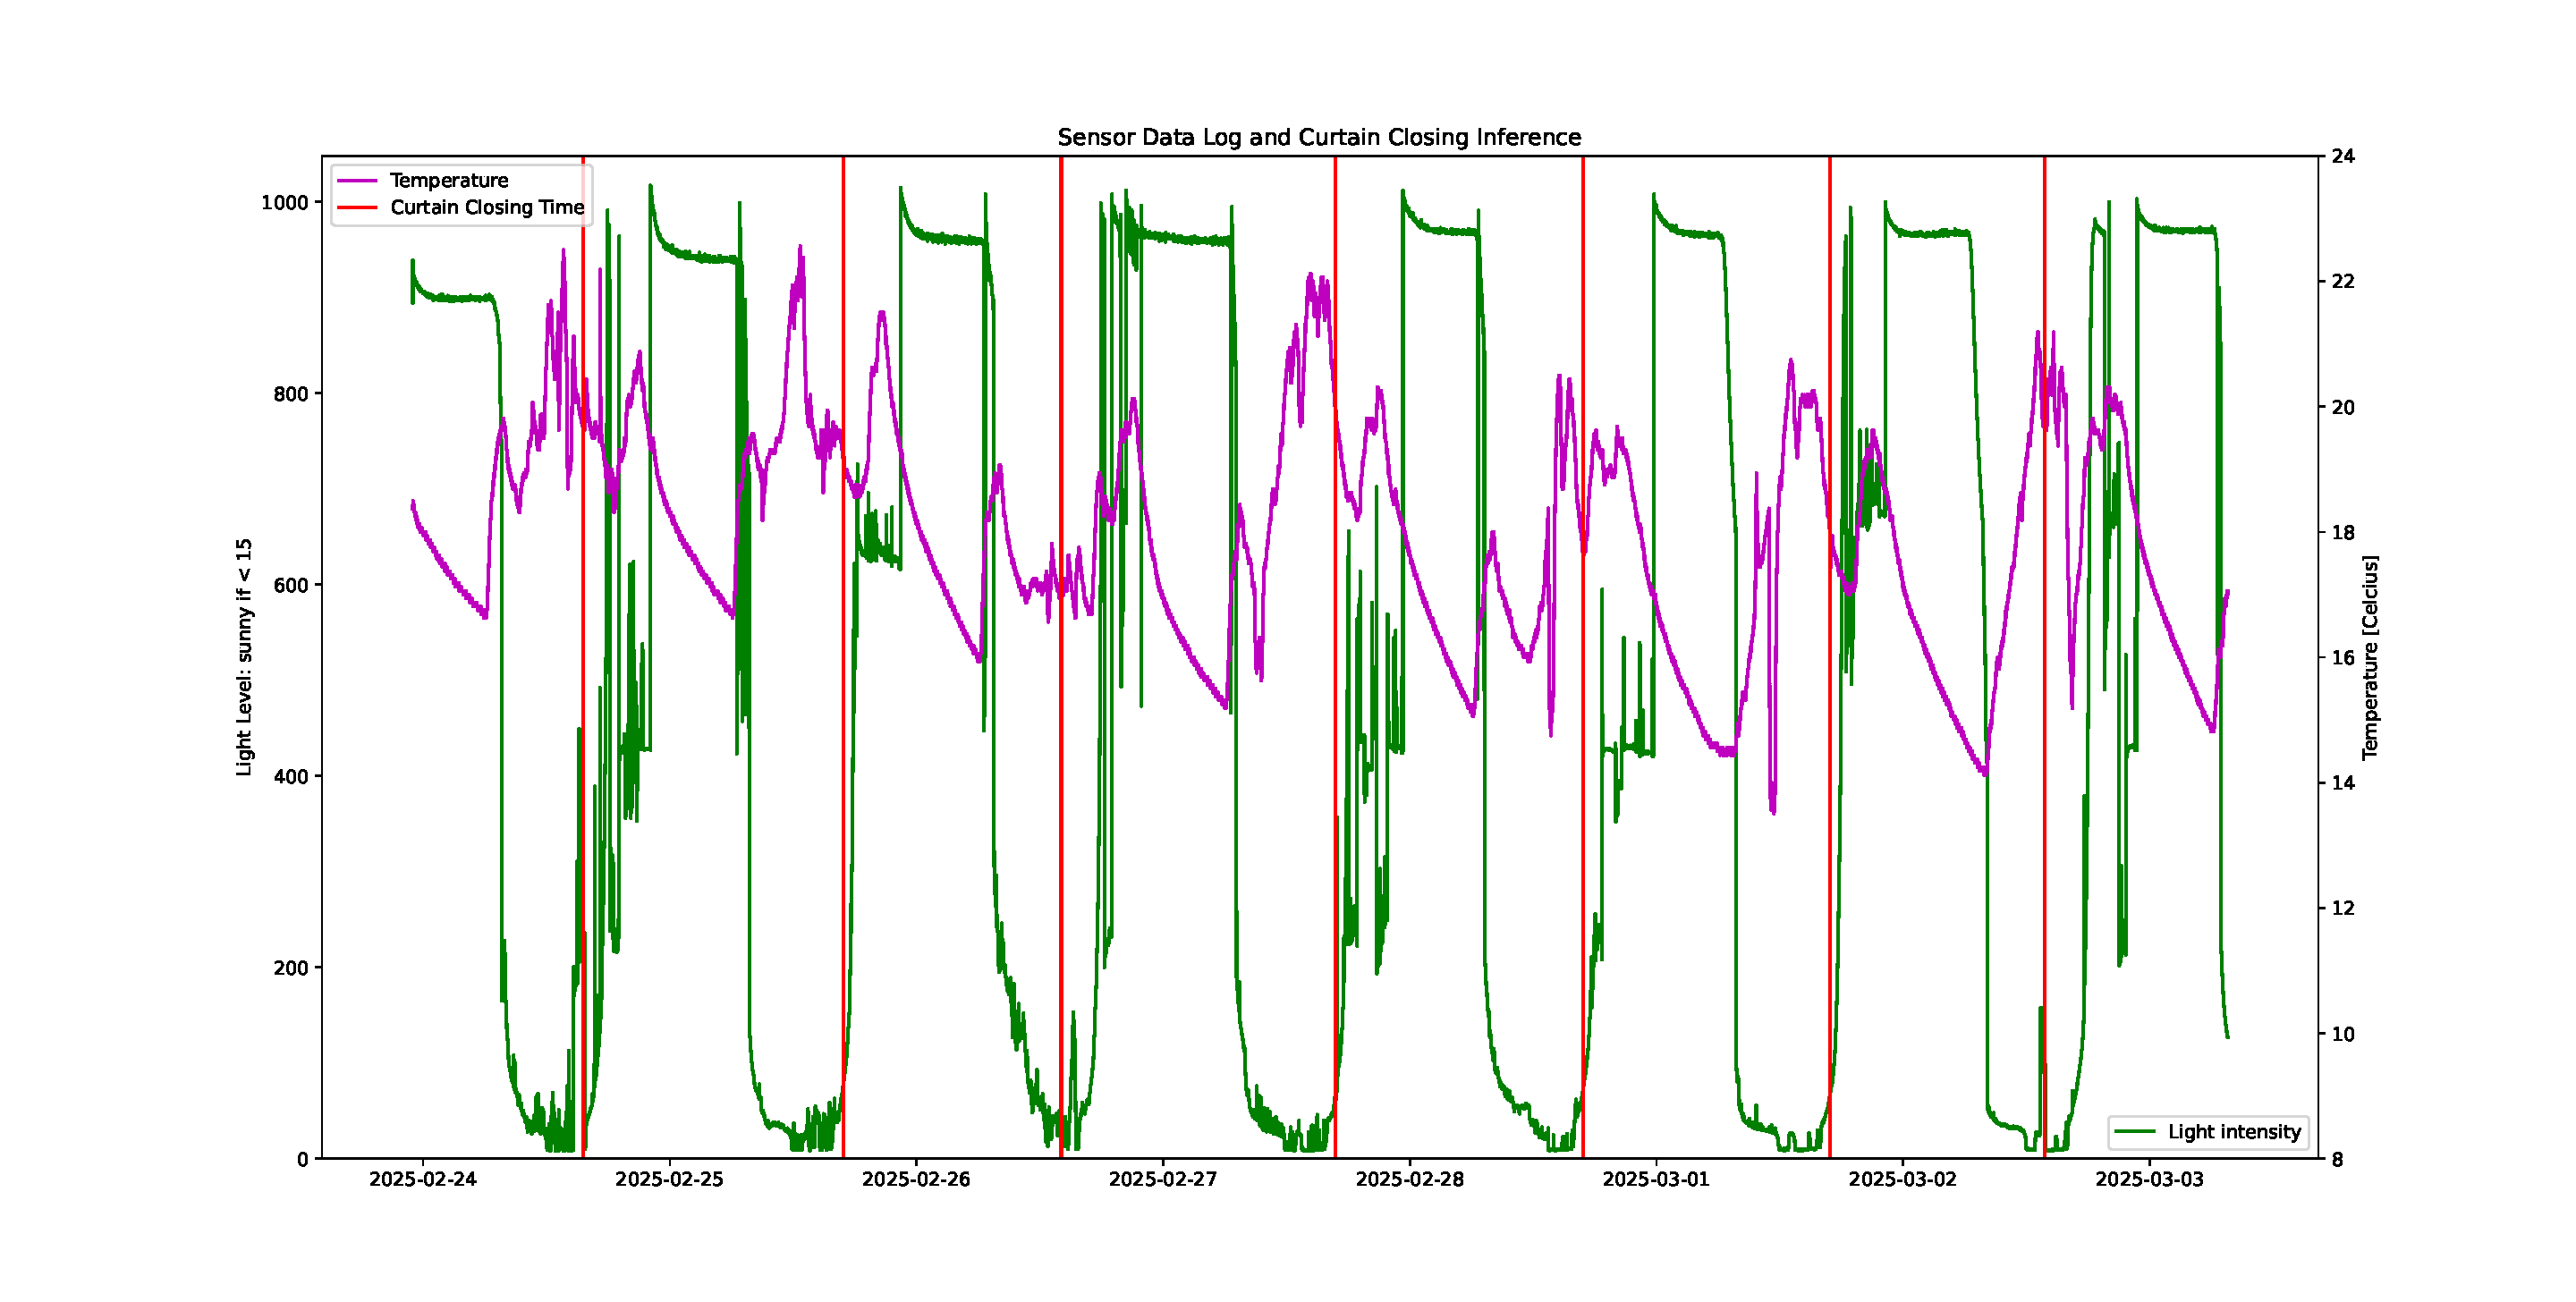
\includegraphics[width=\linewidth]{./figures/logDataPlot.pdf}
    \caption{Temperature and light levels logged from 24 February 2025 to 3 March 2025. Ticks on the x-axis indicate midnight of each day.
    Vertical orange lines indicate for each day the time of conditions for 
    curtain closing being met, i.e., temperature dropping for 30 minutes and light levels too low for effective solar heating. Note that temperature 
    is rising in early mornings (6-8 am) and evenings (5-9pm) following conventional heating system activation. }  
    \label{fig:plot1}
  \end{figure}

To easily view the data and possibly develop the data, it is necessary to plot the data. 
Figure \ref{fig:plot1} displays logged data for a range of days in winter of 2025.
Plots were generated from the logged data using pandas and matplotlib libraries, with the following program:

\begin{lstlisting}
import pandas as pd
from pandas import read_csv
from pandas import DataFrame
from pandas import Grouper
from matplotlib import pyplot

cols2read = ["date","time","Column1","Column2"]

closingTimeData = read_csv("closingTimes.txt", usecols=[0], names=["datetime"], parse_dates=[0])
print(closingTimeData)

series = read_csv('20250223.csv', header=0, parse_dates=[0],usecols=cols2read)  #, index_col=0)
print(series.head())

series["pandasdatetime"]=pd.to_datetime([str(date) + ' ' + str(time) for date,time in zip(series["date"],series["time"])])
print(series.head())

print(f"Time loc {series.columns.get_loc("time")}")

X = series["pandasdatetime"] #series.index

Y1=series['Column1']
Y2=series['Column2']


fig, ax1 = pyplot.subplots(figsize=(10,6))
ax2 = ax1.twinx()

ax1.plot(X, Y1, 'g', label='Light intensity')
ax2.plot(X, Y2, 'm', label='Temperature')

ax1.set_ylabel("Light Level: sunny if < 15")
ax2.set_ylabel("Temperature [Celcius]")

ax1.set_ylim(0, 1048)
ax2.set_ylim(8, 24)
ax1.legend(loc='lower right')
ax2.legend(loc='upper right')
pyplot.axvline(pd.to_datetime(closingTimeData["datetime"])[0], color = 'r', label = "Curtain Closing Time")
for datetime in pd.to_datetime(closingTimeData["datetime"]):
    pyplot.axvline(datetime, color = 'r')
pyplot.legend(loc='upper left')

pyplot.title("Sensor Data Log and Curtain Closing Inference")

pyplot.show()

\end{lstlisting}


\section{Future Work}

Work in progress includes pulling short range weather forecasts information from OpenMeteo\cite{url:openmeteo} for making better decisions 
about curtain closing times.
We have considered using reinforment learning techniques to automate the system, but these are currently out of scope due to lack of training 
data and time.

\begin{thebibliography}{99}

    \bibitem{url:energyUse} 2023 UK greenhouse gas emissions, provisional figures \url{https://assets.publishing.service.gov.uk/media/6604460f91a320001a82b0fd/uk-greenhouse-gas-emissions-provisional-figures-statistical-release-2023.pdf}

    \bibitem{url:solarConstant} Solar Constant \url{https://en.wikipedia.org/wiki/Solar\_constant\#Apparent\_magnitude} (retrieved: 1 March 2025)

    \bibitem{url:solarEnergyStore} \url{https://solar-energy-store.co.uk/off-grid-solar-pv-kits/2kw-2000w-solar-panel-pv-kit-system-for-off-grid-hybrid-self-storage-battery-storage-premium/}

    \bibitem{url:solarVenti} SolarVenti air collectors: \url{https://www.hess-solar.de}

    \bibitem{url:initialCurtainMechanism} Initial curtain opening and closing mechanism: \url{https://www.youtube.com/shorts/H6Un9TCUDxk}

    \bibitem{url:digitalTempSensor} DS18B20 Sensor: \url{https://randomnerdtutorials.com/raspberry-pi-ds18b20-python/}

    \bibitem{url:openmeteo} Open Meteo: \url{https://open-meteo.com/}, accessed on 26 Feb 2025.
        
\end{thebibliography}

\end{document}